%%%%%%%%%%%%%%%%%%%%%%%%%%%%%%%%%%%%%%%%%
% Beamer Presentation
% LaTeX Template
% Version 1.0 (10/11/12)
%
% This template has been downloaded from:
% http://www.LaTeXTemplates.com
%
% License:
% CC BY-NC-SA 3.0 (http://creativecommons.org/licenses/by-nc-sa/3.0/)
%
%%%%%%%%%%%%%%%%%%%%%%%%%%%%%%%%%%%%%%%%%

%----------------------------------------------------------------------------------------
%	PACKAGES AND THEMES
%----------------------------------------------------------------------------------------

\documentclass{beamer}

\mode<presentation> {

% The Beamer class comes with a number of default slide themes
% which change the colors and layouts of slides. Below this is a list
% of all the themes, uncomment each in turn to see what they look like.

%\usetheme{default}
%\usetheme{AnnArbor}
%\usetheme{Antibes}
%\usetheme{Bergen}
%\usetheme{Berkeley}
%\usetheme{Berlin}
%\usetheme{Boadilla}
%\usetheme{CambridgeUS}
%\usetheme{Copenhagen}
%\usetheme{Darmstadt}
%\usetheme{Dresden}
%\usetheme{Frankfurt}
%\usetheme{Goettingen}
%\usetheme{Hannover}
%\usetheme{Ilmenau}
%\usetheme{JuanLesPins}
%\usetheme{Luebeck}
\usetheme{Madrid}
%\usetheme{Malmoe}
%\usetheme{Marburg}
%\usetheme{Montpellier}
%\usetheme{PaloAlto}
%\usetheme{Pittsburgh}
%\usetheme{Rochester}
%\usetheme{Singapore}
%\usetheme{Szeged}
%\usetheme{Warsaw}

% As well as themes, the Beamer class has a number of color themes
% for any slide theme. Uncomment each of these in turn to see how it
% changes the colors of your current slide theme.

%\usecolortheme{albatross}
%\usecolortheme{beaver}
%\usecolortheme{beetle}
%\usecolortheme{crane}
%\usecolortheme{dolphin}
%\usecolortheme{dove}
%\usecolortheme{fly}
%\usecolortheme{lily}
%\usecolortheme{orchid}
%\usecolortheme{rose}
%\usecolortheme{seagull}
%\usecolortheme{seahorse}
%\usecolortheme{whale}
%\usecolortheme{wolverine}

%\setbeamertemplate{footline} % To remove the footer line in all slides uncomment this line
%\setbeamertemplate{footline}[page number] % To replace the footer line in all slides with a simple slide count uncomment this line

%\setbeamertemplate{navigation symbols}{} % To remove the navigation symbols from the bottom of all slides uncomment this line
}
\usepackage[brazil]{babel} % pacote portugues brasileiro
\usepackage[utf8]{inputenc} % pacote para acentuacao direta
\usepackage{graphicx} % Allows including images
\usepackage{booktabs} % Allows the use of \toprule, \midrule and \bottomrule in tables

%----------------------------------------------------------------------------------------
%	TITLE PAGE
%----------------------------------------------------------------------------------------

\title{Um Modelo Conceitual para Cenários de Acidentes em Atividades de Manutenção} % The short title appears at the bottom of every slide, the full title is only on the title page

\author{Jonathan M. Samara \\ Orientador Prof. Dr. Cesar A. Tacla} % Your name
\institute[UTFPR] % Your institution as it will appear on the bottom of every slide, may be shorthand to save space
{
Universidade Tecnológica Federal do Paraná \\ % Your institution for the title page
\medskip
}
\date{\today} % Date, can be changed to a custom date

\begin{document}

\begin{frame}
\titlepage % Print the title page as the first slide
\end{frame}

\begin{frame}
\frametitle{Introdução} % Table of contents slide, comment this block out to remove it
	\begin{itemize}
			\item \textbf{Motivação}: Averiguar modelos que possam ser aplicados a sistemas multiagentes, criar um modelo conceitual sobre um dado estudo de caso e compreender a relação deste com aqueles. 
			\item \textbf{Relevância}: Apresentar um modelo conceitual que defina em termos de classes e relacionamentos uma estrutura lógico-descritiva de fatores ambientais e organizacionais.    
	\end{itemize}
\end{frame}


\begin{frame}
\frametitle{Introdução - Objetivo Geral} % Table of contents slide, comment this block out to remove it
	\begin{itemize}
		\item Sintetizar, construir e avaliar, por intermédio de observações, de análises de documentos técnicos, de análises de modelos computacionais e de entrevista com profissionais da área, um modelo conceitual que define os conceitos e as relações para representar os cenários de ambientes de atividades, bem como os respectivos acidentes que neles podem acontecer, em que a validação ocorre por verificar se os raciocínios (para um dado estudo de caso do setor de energia elétrica) resultantes desse modelo são correspondentes com a realidade a fim de levantar um entendimento formal do problema para a comunidade acadêmica no que tange a que tipo de representação computacional é mais apropriada para determinado contexto. 
	\end{itemize}
\end{frame}

\begin{frame}
\frametitle{Introdução - Objetivos Específicos}
	\begin{enumerate}
    	\item Identificar os aspectos relevantes que devem fazer parte da estrutura do modelo em relação aos 	riscos e consequências (acidentes) para os atores e atividades, que sejam relevantes na prática da 	atividade de manutenção, em caso de falha na operação. 
    	\item Construir um modelo conceitual que seja implementável computacionalmente e que produza as 	inferências que tratem aspectos relevantes ao problema.
    	\item Avaliar o modelo por aplicá-lo a um dado estudo de caso a fim de averiguar se os raciocínios 	produzidos nessa situação estão de acordo com a realidade.  
    	\item Analisar modelos computacionais em relação ao modelo conceitual desse estudo a fim de ter um 	levantamento formal do estado do problema. 
	\end{enumerate}
\end{frame}


\begin{frame}
\frametitle{Fundamentação Teórica - Agentes}
	\begin{itemize}
		\item Um agente é um sistema computacional que está situado em um dado ambiente e que apresenta comportamento autônomo com a finalidade de atingir um dado objetivo que a ele é designado. 
		\item Um agente pode ser estruturado em termos \textit{goal-governed} e \textit{goal-oriented}.
		\item Os agentes \textit{goal-governed} têm capacidades cognitivas e podem representar os seus respectivos objetivos. 
		\item Os agentes \textit{goal-oriented} são programados para alcançar um dado objetivo. 
		\item Artefatos não se enquadram nessas duas características. Essas entidades são exploradas pelo agente para que eles possam alcançar um dado objetivo. 
	\end{itemize}
\end{frame}

\begin{frame}
\frametitle{Fundamentação Teórica - SMA}
	\begin{itemize}
		\item Um sistema multiagente é constituído por agentes autônomos que interagem visando um propósito em comum tendo como consequência um comportamento global. 
		\item Uma organização com essas características, portanto, apresenta em comum; cultura, memória, história, distribuição de atividades e capacidade de distinguir um agente em específico. 
		\item Uma organização de sistema multiagente deve conter relações sociais no que tange a agentes, institutos específicos e grupos sociais. 
		\item Por ser uma organização, uma \textit{SMA} apresenta; Divisão de tipos de atividades, integração, composição, estabilidade/flexibilidade, coordenação, recursividade, representação multinível e causalidade, potenciais e diferenciais, regras e gramáticas.
	\end{itemize}
\end{frame}

\begin{frame}
	\frametitle{Fundamentação Teórica - Normas}
	\begin{figure}[H]
	  \centering
	  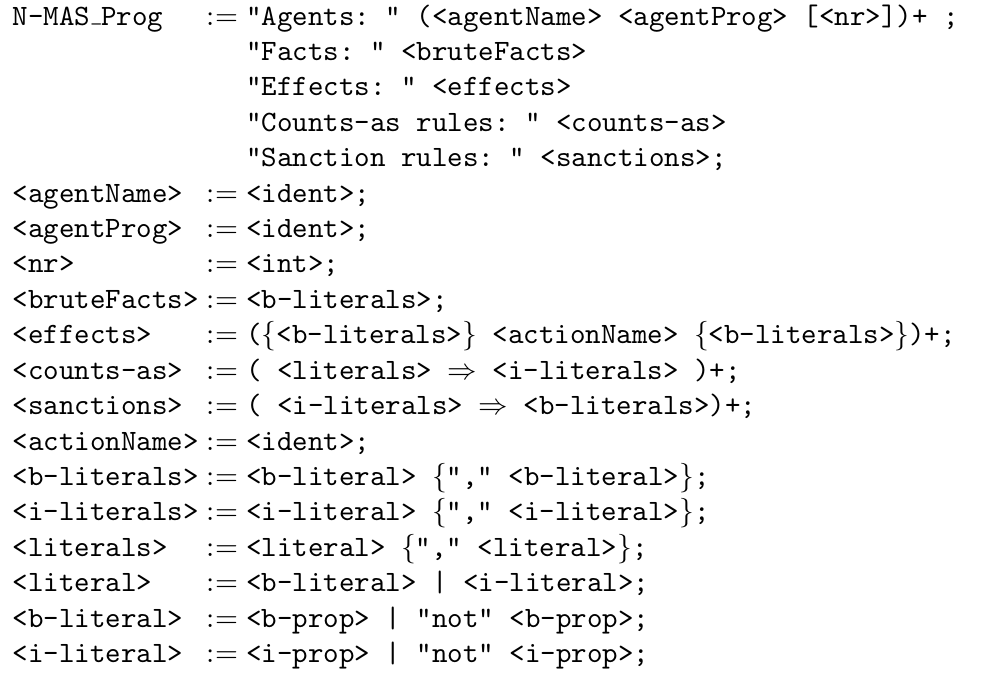
\includegraphics[width=0.5\linewidth]{figure/masprogram.png} 
	  \caption{Linguagem para descrever um programa de multiagentes normativos com a possibilidade de violações e sanções na notação EBNF segundo o texto \cite{dastaniframework}. Nesta notação, $<ident>$ é usado para denotar uma \textit{string} e $<int>$ inteiros. Os termos $<b-prop>$ e $<i-prop>$ são usados para designar dois tipos de conjuntos de proposições que são disjuntos entre si}
	  \label{descreveprograma}
	\end{figure}
\end{frame}


\begin{frame}
	\frametitle{Fundamentação Teórica - Riscos}
	\begin{itemize}
		\item BATU - \textit{Boundary Activities Tolerated during Use} (Atividades Limites Toleradas Durante o Uso). Muitas vezes a equipe adota atividades paliativas a fim de otimizar os processos de produção. Isso envolve assumir níveis de tolerância no que diz respeito ao desempenho e a segurança. 
		\item BCTU - \textit{Boundary Conditions Tolerated by Use} (Condições Limites Toleradas Durante o Uso). O termo condição faz referência a uma situação, um estado, circunstâncias externas às quais pessoas ou até mesmo entidades são afetados no que diz respeito a uma certa decisão atrelada a circunstâncias ambientais, materiais, humanas, de produtos e entre outras.
	\end{itemize}
\end{frame}

\begin{frame}
	\frametitle{Metodologia}
	\begin{itemize}
		\item \textbf{Revisão Exploratória e Análise de Campo}: Estudo de Manuais Técnicos, conversas com profissionais da área, entrevista com Engenheiro de Manutenção, acompanhamento de um procedimento de manutenção em liha viva, criação de textos descrevendo os cenários, participação em Workshops e revisão bibliográfica exploratória.
		\item \textbf{Formalização de um Modelo Conceitual}: Verificar conceitos e seus respectivos relacionamentos. Após isso, escrever essa estrutura em termos de Conjuntos e Relações. Uma ver identificado isso, descrever regras que definem a transitividade do modelo. 
		\item \textbf{Explorar os Arcabouços Possíveis}: Verificar correspondência com outros arcabouços da área de multiagentes e acidentes de trabalho.
		\item \textbf{Aplicação em Estudo de Caso}: Aplicação do modelo conceitual em um dado estudo descaso a fim de verificar a correspondência com a realidade.
	\end{itemize} 
\end{frame}


\begin{frame}
	\frametitle{Resultados - Revisão Exploratória e Análise de Campo}
	\begin{enumerate}
		\item Os trabalhadores que executam os procedimentos.
		\item Os diferentes papéis (ou funções) desses trabalhadores.
		\item As ferramentas usadas pelos profissionais.
		\item Os equipamentos que são submetidos a manutenção.
		\item As interações entre todo tipo de entidade tais como trabalhadores, ferramentas e equipamentos.
		\item As etapas das tarefas que devem ser finalizadas. 
		\item As relações entre todas as entidades e interações com as tarefas
		\item Averiguar a incerteza presente em certos processos e equipamentos que podem gerar acidentes.
		\item Análise das Medidas que são tomadas pelos profissionais para lidar com essas incertezas.
		\item Análise de Cenários onde Profissionais tomam medidas em desacordo com a segurança.
		\item Análise dos riscos gerados a todos.
		\item Análise da possibilidade de algum acidente ocorrer.
	\end{enumerate}
\end{frame}

\begin{frame}
	\frametitle{Resultados - Revisão Exploratória e Análise de Campo}
 	\begin{enumerate}
		\item MOISE+
		\item Modelo de Agentes Normativos de Dastani
		\item V3S 
		\item NormMAS
	\end{enumerate}
\end{frame}

\begin{frame}
	\frametitle{Resultados - Estrutural Conceitual - Módulos}
	\begin{figure}[H]
  		\centering
  			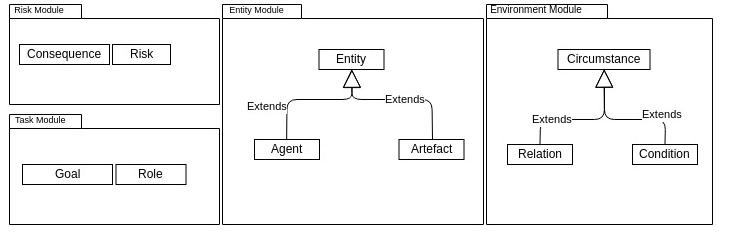
\includegraphics[width=1\linewidth]{../dissertacao/figure/Module.jpeg} 
  		\caption{A estrutura geral das classes do modelo}
  		\label{module}
	\end{figure}
\end{frame}

\begin{frame}
	\frametitle{Resultados - Estrutural Conceitual - Predicados}
	\begin{figure}[H]
  		\centering
  		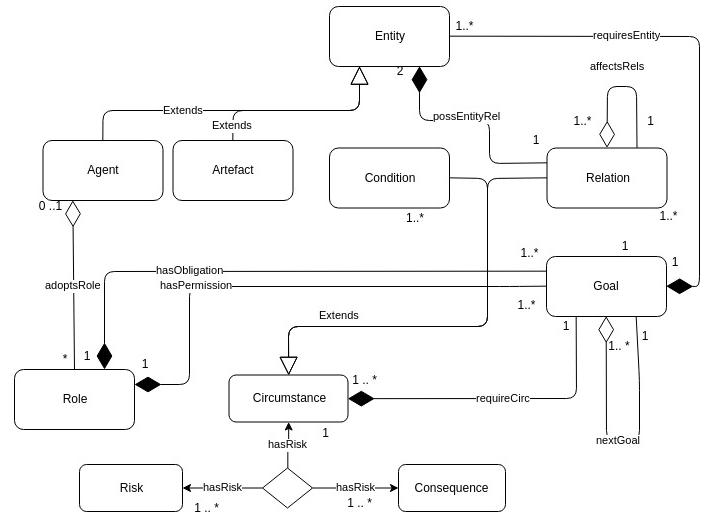
\includegraphics[width=0.8\linewidth]{../dissertacao/figure/Class.jpeg} 
  		\caption{Diagrama de classes do Modelo}
  		\label{classdiagrama}
	\end{figure}
\end{frame}

\begin{frame}
	\frametitle{Resultados - Regras}
	\begin{eqnarray}\label{violationrelation}\nonumber
		hasObligation(\rho_m,g_j) \to hasPermission(\rho_m,g_j), \nonumber \\
    	\rho_m \in Role \wedge g_j \in Goal
	\end{eqnarray}
	\begin{eqnarray}\label{violationentity}\nonumber
		requiresCirc(g_i,c_k) \wedge \neg isPresent(c_k) \wedge  instanceOfCond(c_k) \nonumber \\ 
		\wedge  starts(ag_m,g_i)  \to conditionViol(ag_m,g_i,c_k) \nonumber \\  
    	g_i \in Goal, c_k \in Condition, ag_m \in Agent
	\end{eqnarray}
	\begin{eqnarray}\label{relationViol}\nonumber
		requiresCirc(g_i,r_k)\wedge \neg isPresent(r_k) \wedge instanceOfRel(r_k) \nonumber \\ 
		\wedge starts(ag_m,g_i) \to relationViol(ag_m,g_i,r_k) \nonumber \\  
    	g_i \in Goal, r_k \in Relation, ag_m \in Agent
	\end{eqnarray}
	\begin{eqnarray}\label{entityViol}\nonumber
		requiresEntity(g_i,eg_n) \wedge \neg isPresent(e_k) \wedge starts(ag_m,g_i) \to \nonumber \\ 
	    entityViol(ag_m,g_i,e_k)  \nonumber \\  
	    g_i \in Goal, e_k \in Entity, ag_m \in Agent
	\end{eqnarray}
\end{frame}
\begin{frame}
	\frametitle{Resultados - Regras}
	\begin{eqnarray}\label{consconditionViol}\nonumber
		conditionViol(ag_m,g_i,c_k)  \wedge hasRisk(c_k,risk_j,cs_m) \to \nonumber \\ 
		negConseqFor(g_i,ag_m,risk_j,cs_m) \nonumber \\ 
    	ag_m \in Agent, g_i \in Goal, c_k \in Condition, risk_k \in Risk, cs_m \in Consequence
	\end{eqnarray}
	\begin{eqnarray}\label{consrelationViol}\nonumber
		relationViol(ag_m,g_i,r_k) \wedge hasRisk(r_k,risk_j,cs_m) \to \nonumber \\ 
		negConseqFor(g_i,ag_m,risk_j,cs_m) \nonumber \\ 
	    ag_m \in Agent, g_i \in Goal, r_k \in Relation, risk_k \in Risk, cs_m \in Consequence 
	\end{eqnarray}
	\begin{eqnarray}\label{entityViolaffect}
		relationViol(ag_m,g_i,r_k) \wedge affectsRels(r_k,r_n) \to possOfNegConseqFor(r_n)  \nonumber \\
	    ag_m \in Agent, g_i \in Goal, r_k,r_n \in Relation, 
	\end{eqnarray}
	\begin{eqnarray}\label{consvioent}
		entityViol(ag_m,g_i,e_k) \to stopped(g_i) \nonumber \\  
    	ag_m \in Agent, g_i \in Goal, e_k \in Entity \\ \nonumber
	\end{eqnarray}
\end{frame}

\begin{frame}
	\frametitle{Resultados - Regras}
	\begin{eqnarray}\label{paybutiamnotguilty}
		possOfNegConseqFor(r_k) \wedge  happensNegConseqFor(r_k) \wedge \nonumber \\
		requiresCirc(g_i,r_k) \wedge instanceOfRel(r_k) \wedge \nonumber \\ 
		hasRisk(r_k,risk_j,cs_m) \wedge starts(ag_m,g_i) \nonumber \\ 
		\to negConseqFor(g_i,ag_m,risk_j,cs_m) \nonumber \\ 
	    r_k \in Relation, g_i \in Goal, risk_k \in Risk, cs_m \in Consequence
	\end{eqnarray}
	 \begin{eqnarray}\label{badcons}
		negConseqFor(g_k,ag_m,risk_j,cs_m) \to stopped(g_k) \nonumber \\ 
	    g_k \in Goal, risk_j \in Risk, cs_m \in Consequence
	\end{eqnarray}	
\end{frame}

\begin{frame}
	\frametitle{Resultados - Regras}
	\begin{eqnarray}\label{rolenextgoal}
		adoptsRole(ag_n,\rho_m) \wedge hasPermission(\rho_m,g_j) \wedge nextGoal(g_i,g_j) \nonumber \\
	 	\wedge reached(g_i) \to enabledToStart(ag_i,g_j) \nonumber \\
    	ag_i, ag_n \in Agent, \rho_m \in Role, g_j \in Goal, g_i \in Goal
	\end{eqnarray}
	\begin{eqnarray}\label{rolelastgoal}
		adoptsRole(ag_n,\rho_m) \wedge hasPermission(\rho_m,g_i) \wedge lastGoal(g_i,\rho_m) \nonumber \\
		\wedge reached(g_i) \to stopped(g_i) \nonumber \\
		ag_n \in Agent, \rho_m \in Role, g_i \in Goal
	\end{eqnarray}
\end{frame}
\begin{frame}
	\frametitle{Resultados - Regras}
	\begin{figure}[H]
		\centering
		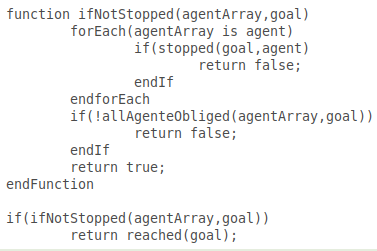
\includegraphics[width=0.6\linewidth]{../dissertacao/figure/algrule6.png} 
		\caption{Condição para definir se um dado objetivo foi atingido ou não} \label{wenStop}  
	\end{figure}
\end{frame}

\begin{frame}
	\frametitle{Resultados - Caso de Estudo}
	\begin{itemize}
		\item O estudo de caso desta pesquisa consiste em sete profissionais de linha viva.
		\item Um supervisor e seis executores.
		\item Céu ensolarado e umidade relativa do ar menor que 70 porcento.
		\item EPI's necessários: capacete, óculos de sol, roupa isolante e antichamas, luvas isolantes e botas isolantes.
		\item  bastão garra de diâmetro 64 x 3600 mm, sela de diâmetro 65, colar, corda de fibra sintética, carretilha, chave com catraca, bastão universal, soquete adequado, locador de pino e bastão com soquete multiangular
		\item O método selecionado para esse tipo de manutenção é a distância.
	\end{itemize}
\end{frame}
\begin{frame}
	\frametitle{Resultados - Raciocínio 1}
	\begin{enumerate}
		\item $adoptsRole(agente4,executor2)$ 
		\item $hasObligation(executor2,g1)$
		\item $requiresCirc(g1,relPanoGlicerina)$
		\item $instanceOfRel(relPanoGlicerina)$ 
		\item $relPanoCorda \in rg1$
		\item $ x = agente4 $
		\item $starts(agente4,g1)$
		\item $affectsRels(relPanoGlicerina,relBastaoGarraCondutor)$
		\item $affectsRels(relPanoGlicerina,relCordaEstropo)$  
		\item $affectsRels(relPanoGlicerina,relChaveCatracaParafuso)$
		\item $affectsRels(relPanoGlicerina,relParafusoConector)$ 
		\item $affectsRels(relPanoGlicerina,relSoqueteParafuso)$ 
		\item $affectsRels(relPanoGlicerina,relAgente4Corda)$ 
		\item $affectsRels(relPanoGlicerina,relEstropoCorda)$	
	\end{enumerate}
\end{frame}
\begin{frame}
	\frametitle{Resultados - Raciocínio 1}
	\begin{eqnarray}\nonumber
		requiresCirc(g1,relPanoGlicerina) \wedge \nonumber \\  
		\neg isPresent(relPanoGlicerina) \wedge \nonumber \\   
		instanceOfRel(relPanoGlicerina) \wedge \nonumber \\   
		starts(agente4,g1) \to \nonumber \\
		relationViol(agente4,g1,relPanoGlicerina) \nonumber \\  
	\end{eqnarray}
	\begin{eqnarray} \nonumber
		relationViol(agente4,g1,relPanoGlicerina) \nonumber \\
		\wedge affectsRels(relPanoGlicerina,relEstropoCorda) \nonumber \\
    	\to possOfNegConseqFor(relEstropoCorda) \nonumber \\
	\end{eqnarray}

	O mesmo ocorre para as demais relações.
\end{frame}
\begin{frame}
	\frametitle{Resultados - Raciocínio 2}
	\begin{enumerate}
		\item $adoptsRole(agente2,executor1)$ 
		\item $adoptsRole(agente3,executor1)$	 	
		\item $adoptsRole(agente4,executor2)$	 
		\item $hasObligation(executor1,g1)$
		\item $hasObligation(executor2,g1)$
		\item $starts(agente2,g1)$ 
		\item $starts(agente3,g1)$	 	
		\item $starts(agente4,g1)$	
		\item $requiresEntity(g1,pano)$		
		\item $\neg isPresent(pano)$
	\end{enumerate}
\end{frame}
\begin{frame}
	\frametitle{Resultados - Raciocínio 2}
	\begin{eqnarray}\nonumber
		requiresEntity(g1,pano) \wedge \neg isPresent(pano) \wedge starts(agente2,g1)  \nonumber \\ 
		\to entityViol(agente2,g1,pano) \nonumber \\ 	    
	\end{eqnarray}

	\begin{eqnarray}\nonumber
		requiresEntity(g1,pano) \wedge \neg isPresent(pano) \wedge starts(agente3,g1) \nonumber \\ 
	    \to entityViol(agente3,g1,pano) \nonumber \\
	\end{eqnarray}
	\begin{eqnarray}\nonumber
		requiresEntity(g1,pano) \wedge \neg isPresent(pano) \wedge starts(agente4,g1) \nonumber \\ 
	    \to entityViol(agente4,g1,pano)  \nonumber \\	
	\end{eqnarray}
	\begin{eqnarray}
		entityViol(agente4,g1,pano) \to stopped(g1)
	\end{eqnarray}
\end{frame}

\begin{frame}
	\frametitle{Resultados - Raciocínio 3}
	\begin{enumerate}
		\item $adoptsRole(agente5,executor3)$
		\item $hasObligation(executor3,g11)$	
		\item $starts(agente5,g11)$ 
		\item $requiresCirc(g11,umidade70)$
		\item $isIstanceOfCond(umidade70)$
		\item $\neg isPresent(umidade70)$
		\item $hasRisk(umidade70,eletrocutado,morte)$
	\end{enumerate}
\end{frame}

\begin{frame}
	\frametitle{Resultados - Raciocínio 3}
	\begin{eqnarray}\nonumber
		requiresCirc(g11,umidade70) \wedge \neg isPresent(umidade70) \\ \nonumber
		\wedge instanceOfCond(umidade70) \wedge starts(agente5,g11)  \to \\ \nonumber   
		conditionViol(agente5,g11,umidade70) \nonumber \\	
	\end{eqnarray}
	\begin{eqnarray} \nonumber
		conditionViol(agente5,g11,umidade70) \wedge hasRisk(umidade70,eletrocutado,morte) \nonumber \\ 
		\to negConseqFor(g11,agente5,eletrocutado,morte) \nonumber \\ 	
	\end{eqnarray}
	\begin{eqnarray}
		negConseqFor(g11,agente5,eletrocutado,morte) \to stopped(g11)
	\end{eqnarray}

\end{frame}

\begin{frame}
	\frametitle{Resultados - Raciocínio 4}
	\begin{enumerate}
		\item $adoptsRole(agente4,executor2)$
		\item $hasObligation(executor4,g15)$	
		\item $starts(agente4,g15)$ 
		\item $requiresCirc(g15,relChaveCatracaParafuso)$
		\item $isInstanceOfRel(relChaveCatracaParafuso)$	
		\item $\neg isPresent(relChaveCatracaParafuso)$
		\item $hasRisk(relChaveCatracaParafuso,eletrocutado,morte)$
	\end{enumerate}
\end{frame}

\begin{frame}
	\frametitle{Resultados - Raciocínio 4}
	\begin{eqnarray} \nonumber
		requiresCirc(g15,relChaveCatracaParafuso)\wedge  \nonumber \\
		\neg isPresent(relChaveCatracaParafuso) \wedge \nonumber \\
		instanceOfRel(relChaveCatracaParafuso) \wedge starts(agente4,g15) \to \nonumber \\
		relationViol(agente4,g15,relChaveCatracaParafuso)
	\end{eqnarray}
	\begin{eqnarray}\nonumber
		relationViol(agente4,g15,relChaveCatracaParafuso) \nonumber \\ 
		 \wedge hasRisk(relChaveCatracaParafuso,eletrocutado,morte) \to \nonumber \\ 
		negConseqFor(g15,agente4,eletrocutado,morte)
	\end{eqnarray}	
	\begin{eqnarray}
		negConseqFor(g15,agente4,eletrocutado,morte) \to stopped(g15)
	\end{eqnarray}
\end{frame}

\begin{frame}
	\frametitle{Resultados - Raciocínio 5}
	\begin{enumerate}
		\item $requiresCirc(g19,relParafusoConector)$		
		\item $hasObligation(executor3,g19)$
		\item $hasObligation(executor4,g19)$
		\item $hasObligation(executor5,g19)$		
		\item $starts(agente5,g19)$
		\item $starts(agente6,g19)$
		\item $starts(agente7,g19)$									
		\item $adoptsRole(agente5,executor3)$
		\item $adoptsRole(agente6,executor4)$
		\item $adoptsRole(agente7,executor5)$
		\item $hasRisk(relParafusoConector,eletrocutado,morte)$
		\item $possOfNegConseqFor(relParafusoConector)$
		\item $happensNegConseqFor(g19,relParafusoConector)$	
	\end{enumerate}
\end{frame}

\begin{frame}
	\frametitle{Resultados - Raciocínio 5}
	\begin{eqnarray}\nonumber
	   possOfNegConseqFor(relParafusoConector) \nonumber \\
	    \wedge happensNegConseqFor(relParafusoConector) \nonumber \\ 
	    \wedge requiresCirc(g19,relParafusoConector) \nonumber \\  
	    \wedge instanceOfRel(relParafusoConector) \nonumber \\ 
	    \wedge hasRisk(relParafusoConector,eletrocutado,morte) \nonumber \\  
	    \wedge starts(agente5,g19) \nonumber \\ 
	    \to negConseqFor(g19,agente5,eletrocutado,morte) \\ \nonumber    
	\end{eqnarray}	
	\begin{eqnarray}
		negConseqFor(g19,agente5,eletrocutado,morte) \to stopped(g19)
	\end{eqnarray}
	O mesmo para o agente6 e agente7.
\end{frame}

\begin{frame}
	\frametitle{Resultados - Raciocínio 6}
	\begin{enumerate}
		\item $stopped(agente2) \to F$	
		\item $stopped(agente3) \to F$
		\item $stopped(agente4) \to F$
		\item $stopped(agente5) \to F$
		\item $stopped(agente7) \to F$
		\item $hasObligation(executor1,g23)$	
		\item $hasObligation(executor2,g23)$	
		\item $hasObligation(executor3,g23)$		
		\item $adoptsRole(agente2,executor1)$
		\item $adoptsRole(agente3,executor1)$
		\item $adoptsRole(agente4,executor2)$
		\item $adoptsRole(agente5,executor3)$
		\item $adoptsRole(agente7,executor5)$
	\end{enumerate}
\end{frame}
\begin{frame}
	\frametitle{Resultados - Raciocínio 6}
	\begin{itemize}
		\item $ag_{array} = \{ agente2,agente3,agente4,agente5,agente7 \}$
		\item $stopped(goal,Agente) \to F$ para todos os agentes		
		\item $allAgentObligate(ag_{array},goal) \to T$
		\item $ifNotStopped(ag_{array},goal) \to T$
		\item $reached(goal) \to T$
	\end{itemize}
\end{frame}
\begin{frame}
	\frametitle{Discussão - Critérios de Comparação}
	\begin{itemize}
		\item \textbf{Agente} condiz numa representação dos estados internos que um agente pode ter
		\item O critério \textbf{SMA} condiz na presença de elementos que são necessário para especificar um \textit{Sistema Multiagente}
		\item O critério \textbf{Artefato} condiz com elementos que correspondem ao tratado na Fundamentação Teórica.
		\item \textbf{Norma} corresponde a regras que devem ser acatadas pelos agentes 
		\item \textbf{Violação} define o que corresponde o não cumprimento de uma dada regra
		\item \textbf{Sanção} implica penalidade que está sobre o agente.
		\item \textbf{Risco} consiste no evento ruim que tem um dado potencial de ocorrer sobre o agente
	\end{itemize}
\end{frame}
\begin{frame}
	\frametitle{Discussão - Critérios de Comparação}
	\begin{itemize}
		\item \textbf{P.O.A.E} significa Possibilidade de Ocorrer algo Errado.
		\item \textbf{Objetivos} implica alvos que devem ser atingidos pelos agentes 
		\item \textbf{C.A} consiste em condições ambientes que interagem com a atividade executada pelos agentes.
		\item \textbf{I.AG.AR} representa as interações entre agentes e artefatos
		\item \textbf{D.C.A} - Descrição de Cenários de Acidentes, consiste na capacidade de desenvolver raciocínios a fim de representar cenários de acidentes.
	\end{itemize}
\end{frame}
\begin{frame}
	\frametitle{Discussão - Expressividade}
	\begin{itemize}
			\item nenhuma - o engenheiro de modelagem terá de criar uma estrutura conceitual grande e complexa. 
			\item pouco - possui algumas estruturas pré-definidas que diminuem o esforço da especificação. 
			\item expressivo - o modelo permite especificar o objeto de interesse sem que o engenheiro tenha de criar muitos atributos para o domínio de interesse.
			\item muito expressivo - o modelo apresenta diversos conceitos específicos para representar o objeto em interesse
			\item altamente expressivo - o modelo especifica o objetivo de interesse muito bem fazendo com que o engenheiro de conhecimento não tenha que definir nenhum critério conceitual a mais.
	\end{itemize}
\end{frame}
\begin{frame}
	\frametitle{Discussão - Análise Comparativa}
	\begin{table}[H]
	    \centering
	    \begin{tabular}{|l|l|l|l|l|}
	        \hline
	        \textbf{Critérios} & \textbf{MOISE+}        & \textbf{DASTANI}	\\ \hline
	        \textbf{Agente}    & pouco                  & pouco             \\ \hline
	        \textbf{SMA}       & altamente              & pouco             \\ \hline
	        \textbf{Artefato}  & nenhuma                & pouco             \\ \hline
	        \textbf{Norma}     & nenhuma                & altamente			\\ \hline
	        \textbf{Violação}  & nenhuma                & altamente         \\ \hline
	        \textbf{Sanção}    & nenhuma                & altamente         \\ \hline
	        \textbf{Risco}     & nenhuma                & pouco             \\ \hline
	        \textbf{P.O.A.E}   & nenhuma                & pouco             \\ \hline
	        \textbf{Objetivos} & muito                  & pouco             \\ \hline
	        \textbf{C.A}       & nenhuma                & pouco             \\ \hline
	        \textbf{I.AG.AR}   & nenhuma                & pouco             \\ \hline
	        \textbf{D.C.A}     & nenhuma                & pouco				\\ \hline
	    \end{tabular}
	\end{table}	
\end{frame}

\begin{frame}
	\frametitle{Discussão - Análise Comparativa}
	\begin{table}[H]
		\centering
		\begin{tabular}{|l|l|l|l|l|}
			\hline
			\textbf{Critérios}     & \textbf{V3S}         & \textbf{NORMMAS}          \\ \hline
			\textbf{Agente}        & muito                & pouco                     \\ \hline
			\textbf{SMA}           & expressivo           & pouco                     \\ \hline
			\textbf{Artefato}      & expressivo           & pouco                     \\ \hline
			\textbf{Norma}         & pouco                & altamente                 \\ \hline
			\textbf{Violação}      & pouco                & altamente                 \\ \hline
			\textbf{Sanção}        & pouco                & altamente                 \\ \hline
			\textbf{Risco}         & altamente            & pouco                     \\ \hline
			\textbf{P.O.A.E}       & pouco                & pouco                     \\ \hline
			\textbf{Objetivos}     & muito                & pouco                     \\ \hline
			\textbf{C.A}           & pouco                & pouco                     \\ \hline
			\textbf{I.AG.AR}       & pouco                & pouco                    \\ \hline
			\textbf{D.C.A}         & altamente            & pouco					\\ \hline
		\end{tabular}
	\end{table}
\end{frame}


\begin{frame}
	\frametitle{Discussão - Consistência dos Resultados - Caso de Estudo}
	\begin{itemize}
		\item  O caso em análise cumpre com os interesses da pesquisa pois apresenta um cenário onde profissionais usam ferramentas para trabalhar de forma colaborativa a fim de atingir um determinado objetivo
		\item Os profissionais são expostos a um dado risco e podem sofrer acidentes que advêm tanto de responsabilidade própria bem como responsabilidade do outro.
		\item A compreensão da atividade propriamente dita não foi uma tarefa fácil e exigiu grande esforço do autor
		\item O caso de estudo em análise é um cenário que é totalmente possível de ser factual, contudo existe diversas outras possibilidades de organizar a mesma manutenção.
	\end{itemize}
\end{frame}


\begin{frame}
	\frametitle{Discussão - Consistência dos Resultados - Caso de Estudo}
	\begin{itemize}
		\item A primeira fase consistiu em descrever a manutenção em termos de objetivos que as vezes são organizados em série e as vezes em paralelo
		\item Um ponto  complicado de se verificar nesse estudo se deve ao fato de que os profissionais não precisam executar os objetivos na estrutura em que o modelo foi apresentado.
		\item Há um número finito e relativamente pequeno sobre como esses objetivos podem ser organizados e isso ameniza a falta de previsibilidade de como a manutenção será realizada.
		\item Solução para essa questão; 1 - Engenheiro de Manutenção organiza os objetivos de todas formas possíveis, 2 - Definir todas as relações possíveis que o predicado $nextGoal(g_i,g_j)$ permite em uma única estrutura.
	\end{itemize}
\end{frame}


\begin{frame}
	\frametitle{Discussão - Considerações sobre Critérios Metodológicos ao Estudo de Caso}
	\begin{itemize}
		\item Organização dos Objetivos pode ser modificada pelos profissionais durante a execução das Atividades.
		\begin{itemize}
			\item \textbf{Soluções}: Gerar um modelo para cada cenário, considerar todas as relações possíveis para $nextGoal(g_i,g_j)$ e Usar u algoritmo de \textit{Partial Order Planning}
		\end{itemize}
		\item Não foram considerados todos os riscos para o estudo de casos, assim como as possíveis consequências. Contudo, os riscos e consequências definidos no estudo de caso são os mais prováveis de ocorrer.
		\item $possEntityRel(r_l,e_i,e_k)$ - Permitiu a elaboração de diversos raciocínios, contudo tornou a estrutura do modelo altamente complexa.
		\item $affectsRels(r_k,r_n)$ - Apresenta alto grau de abstração ao modelo. Contudo, simplifica o processo de modelagem.
		\item $requiresCirc(circ_n,g_m)$, $requiresEntity(goal_i, e_j)$, $instanceOfRel(circ_n)$ e $instanceOfCond(circ_n)$ - descrição rigorosa sobre procedimento custoso. 
	\end{itemize}
\end{frame}

\begin{frame}
	\frametitle{Discussão - Considerações sobre Critérios Metodológicos ao Raciocínios}
	\begin{itemize}
		\item 1 e 5 - Descreve a situação onde o erro cometido por um agente gera consequências negativas em outro momento da execução sobre um outro agente. Apesar do alto grau de abstração que $possOfNegConseqFor$ trás a ambos raciocínios, esse predicado torna o modelo mais simples. 
		\item 2 - Descreve exatamente o cenário onde a ausência gera a interrupção de uma dada atividade. Um cenário que não é considerado por esse raciocínio se da na condição dos profissionais adaptarem alguma ferramenta na ausência da ferramenta padrão.
	\end{itemize}
\end{frame}

\begin{frame}
	\frametitle{Discussão - Considerações sobre Critérios Metodológicos ao Raciocínios}
	\begin{itemize}
		\item 3 - Descreve a situação onde um agente morre por cometer uma dada violação de condição. O cenário que esse raciocínio não considera se deve ao fato de que nem toda violação de condição resulta em consequências negativos. Uma forma de corrigir isso consiste em conceber regras com $possOfNegConseqFor$.
		\item 4 - Descreve a seguinte situação: Um profissional usa a chave catraca de forma inapropriada ocasionando a sua morte. Um possível cenário que não é considerado por essa modelagem reside na do profissional simplesmente não conseguir executar a relação, sem que isso resulte em algum acidente.
		\item 6 - Demonstra que o modelo é capaz de interpretar quando um objetivo é encerrado e qual deve ser o próximo passo do agente. 
		\item 7 - Apresenta como o modelo se comporta quando é feito uma consulta que não corresponde a realidade. 
	\end{itemize}
\end{frame}

\begin{frame}
	\frametitle{Conclusão - Reflexão sobre Objetivo}
	\begin{itemize} 
		\item Foi feito estudo de documentos técnicos, foi feito entrevista com Engenheiro de Manutenção, foi feito acompanhamento de documentos técnicos, houve acompanhamento de procedimentos de manutenção em linha viva.
		\item Foi concebido um modelo conceitual.
		\item O modelo conceitual foi aplicado em um estudo de caso. Isso possibilitou formular raciocínios e verificar quais cenários foram representados apropriadamente e quais cenários não foram representados adequadamente.
		\item Houve uma análise da comparativa entre modelos computacionais balizado pelo modelo conceitual definido nesse estudo.
		\item Logo, o Objetivo Geral e os Objetivos Específicos foram atingidos.    
	\end{itemize}
\end{frame}

\begin{frame}
	\frametitle{Conclusão}
	\begin{itemize}
		\item \textit{MOISE+} é mais apropriado para representar os seguintes conceitos: \textit{Agente, SMA, objetivos};
		\item \textit{Dastani} é mais apropriado para representar os seguintes conceitos \textit{Normas, Violações, Sanções};
		\item \textit{V3S} é mais apropriado para representar \textit{SMA, Artefato, Riscos e contém estruturas otimizadas para descrever dinamicamente os cenários de acidentes}
		\item \textit{NORMMAS} é mais apropriado para representar os seguintes conceitos \textit{Normas, Violações, Sanções};
		\item No que tange ao contraste do modelo conceitual proposto nesse estudo em relação aos arcabouços verificados nesse texto, o autor conclui que aquele unifica em uma única estrutura concepções que são tratadas de formas isoladas aos demais modelos computacionais.
	\end{itemize}
\end{frame}

\begin{frame}
	\frametitle{Conclusão}
	\begin{enumerate}
		\item Em vez de trabalhar conceitos de possibilidade, sintetizar um modelo estatístico probabilístico na estrutura conceitual proposta neste estudo.
		\item Investigar novas estruturas conceituais para tratar cenários onde os agentes buscam técnicas alternativas para resolver um determinado problema. 
		\item Investigar novas estruturas conceituais onde uma violação pode ou não gerar uma sanção para as condições ambientes (ou seja, em vez de tratar a possibilidade sobre um relacionamento futuro, tratar a possibilidade sobre um relacionamento presente).
		\item Investigar novas estruturas conceituais que considerem a violação de relacionamento em termos de possibilidades e não de um efeito direto no que tange a uma dada causa.   
	\end{enumerate}
\end{frame}


\end{document} 	